\documentclass[a4paper]{amsart}
\usepackage{a4wide}
\usepackage[]{graphicx}

\setlength{\parindent}{0.0in}
\setlength{\parskip}{0.1in}

\newcommand{\laplace}[1]{\mathcal{L}\{#1\}}
\newcommand{\Hv}{\textrm{H}}
\renewcommand{\b}{\mathbf}

\begin{document}
\title{6G5Z3011 Multi-variable calculus and analytical methods}
\author{Tutorial Sheet 10}
\maketitle

\textbf{Qs 1 -- 4} Further exercises on Fourier series. 

\begin{enumerate}
  \item
Find the Fourier series for the function whose graph is shown below.

\begin{center}
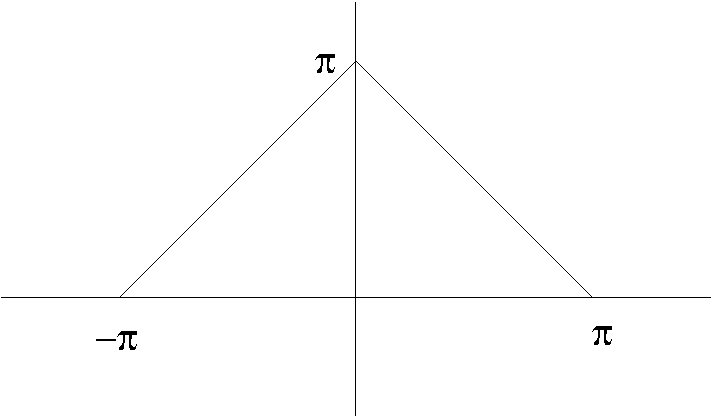
\includegraphics[scale=0.5]{sheet16q1.pdf} 
\end{center}

Sketch the graph of the series over the range $(-4\pi,4\pi)$ and use the series to evaluate the series
$$\sum_{m=1}^\infty \frac{1}{(2m-1)^2}.$$
\item
Using the formulae
$$ \sin A - \sin B = 2 \sin \left ( \frac{A-B}{2} \right ) \cos \left ( \frac{A+B}{2} \right ) ,$$
$$  \cos A - \cos B = 2 \sin \left ( \frac{A+B}{2} \right ) \sin \left ( \frac{A-B}{2} \right ),$$
find the Fourier series of the half way rectified wave $f$ defined by 
$$ f(x) = \left \{ 
\begin{array}{rr}
0,& -\pi < x \leq 0 \\
\sin x , & 0 < x \leq \pi
\end{array} \right.
.$$
Sketch the graph of the series over the interval $(-3\pi,3\pi)$. Use the Fourier series to find the sum of the series 
$$ \sum_{m=1}^\infty \frac{1}{4m^2 -1} .$$
\item
Find the cosine series for the sine function over the interval $(0,\pi)$. Use may be made of the formulae from question (2) above. Sketch the graph of the series over the interval $(-3\pi,3\pi)$.
\item
Use the Fourier series for the function $f$ defined by $f(x)=x$ to obtain Fourier series for the functions defined by $f(x)=x^2$ and $f(x)=x^3$. Hence evaluate the following series
\begin{enumerate}
\item
$$ \sum_{m=1}^\infty \frac{(-1)^{m+1}}{2m-1} $$
\item
$$ \sum_{m=1}^\infty \frac{1}{m^2} $$
\item
$$ \sum_{m=1}^\infty \frac{(-1)^{m+1}}{\left ( 2m-1 \right )^3} $$
\item
$$ \sum_{m=1}^\infty \frac{1}{m^4} $$
\end{enumerate}
\end{enumerate}


\end{document}